% Options for packages loaded elsewhere
\PassOptionsToPackage{unicode}{hyperref}
\PassOptionsToPackage{hyphens}{url}
\PassOptionsToPackage{dvipsnames,svgnames,x11names}{xcolor}
%
\documentclass[
  letterpaper,
  DIV=11,
  numbers=noendperiod]{scrartcl}

\usepackage{amsmath,amssymb}
\usepackage{iftex}
\ifPDFTeX
  \usepackage[T1]{fontenc}
  \usepackage[utf8]{inputenc}
  \usepackage{textcomp} % provide euro and other symbols
\else % if luatex or xetex
  \usepackage{unicode-math}
  \defaultfontfeatures{Scale=MatchLowercase}
  \defaultfontfeatures[\rmfamily]{Ligatures=TeX,Scale=1}
\fi
\usepackage{lmodern}
\ifPDFTeX\else  
    % xetex/luatex font selection
\fi
% Use upquote if available, for straight quotes in verbatim environments
\IfFileExists{upquote.sty}{\usepackage{upquote}}{}
\IfFileExists{microtype.sty}{% use microtype if available
  \usepackage[]{microtype}
  \UseMicrotypeSet[protrusion]{basicmath} % disable protrusion for tt fonts
}{}
\makeatletter
\@ifundefined{KOMAClassName}{% if non-KOMA class
  \IfFileExists{parskip.sty}{%
    \usepackage{parskip}
  }{% else
    \setlength{\parindent}{0pt}
    \setlength{\parskip}{6pt plus 2pt minus 1pt}}
}{% if KOMA class
  \KOMAoptions{parskip=half}}
\makeatother
\usepackage{xcolor}
\setlength{\emergencystretch}{3em} % prevent overfull lines
\setcounter{secnumdepth}{-\maxdimen} % remove section numbering
% Make \paragraph and \subparagraph free-standing
\ifx\paragraph\undefined\else
  \let\oldparagraph\paragraph
  \renewcommand{\paragraph}[1]{\oldparagraph{#1}\mbox{}}
\fi
\ifx\subparagraph\undefined\else
  \let\oldsubparagraph\subparagraph
  \renewcommand{\subparagraph}[1]{\oldsubparagraph{#1}\mbox{}}
\fi


\providecommand{\tightlist}{%
  \setlength{\itemsep}{0pt}\setlength{\parskip}{0pt}}\usepackage{longtable,booktabs,array}
\usepackage{calc} % for calculating minipage widths
% Correct order of tables after \paragraph or \subparagraph
\usepackage{etoolbox}
\makeatletter
\patchcmd\longtable{\par}{\if@noskipsec\mbox{}\fi\par}{}{}
\makeatother
% Allow footnotes in longtable head/foot
\IfFileExists{footnotehyper.sty}{\usepackage{footnotehyper}}{\usepackage{footnote}}
\makesavenoteenv{longtable}
\usepackage{graphicx}
\makeatletter
\def\maxwidth{\ifdim\Gin@nat@width>\linewidth\linewidth\else\Gin@nat@width\fi}
\def\maxheight{\ifdim\Gin@nat@height>\textheight\textheight\else\Gin@nat@height\fi}
\makeatother
% Scale images if necessary, so that they will not overflow the page
% margins by default, and it is still possible to overwrite the defaults
% using explicit options in \includegraphics[width, height, ...]{}
\setkeys{Gin}{width=\maxwidth,height=\maxheight,keepaspectratio}
% Set default figure placement to htbp
\makeatletter
\def\fps@figure{htbp}
\makeatother

\KOMAoption{captions}{tableheading}
\makeatletter
\makeatother
\makeatletter
\makeatother
\makeatletter
\@ifpackageloaded{caption}{}{\usepackage{caption}}
\AtBeginDocument{%
\ifdefined\contentsname
  \renewcommand*\contentsname{Table of contents}
\else
  \newcommand\contentsname{Table of contents}
\fi
\ifdefined\listfigurename
  \renewcommand*\listfigurename{List of Figures}
\else
  \newcommand\listfigurename{List of Figures}
\fi
\ifdefined\listtablename
  \renewcommand*\listtablename{List of Tables}
\else
  \newcommand\listtablename{List of Tables}
\fi
\ifdefined\figurename
  \renewcommand*\figurename{Figure}
\else
  \newcommand\figurename{Figure}
\fi
\ifdefined\tablename
  \renewcommand*\tablename{Table}
\else
  \newcommand\tablename{Table}
\fi
}
\@ifpackageloaded{float}{}{\usepackage{float}}
\floatstyle{ruled}
\@ifundefined{c@chapter}{\newfloat{codelisting}{h}{lop}}{\newfloat{codelisting}{h}{lop}[chapter]}
\floatname{codelisting}{Listing}
\newcommand*\listoflistings{\listof{codelisting}{List of Listings}}
\makeatother
\makeatletter
\@ifpackageloaded{caption}{}{\usepackage{caption}}
\@ifpackageloaded{subcaption}{}{\usepackage{subcaption}}
\makeatother
\makeatletter
\@ifpackageloaded{tcolorbox}{}{\usepackage[skins,breakable]{tcolorbox}}
\makeatother
\makeatletter
\@ifundefined{shadecolor}{\definecolor{shadecolor}{rgb}{.97, .97, .97}}
\makeatother
\makeatletter
\makeatother
\makeatletter
\makeatother
\ifLuaTeX
  \usepackage{selnolig}  % disable illegal ligatures
\fi
\IfFileExists{bookmark.sty}{\usepackage{bookmark}}{\usepackage{hyperref}}
\IfFileExists{xurl.sty}{\usepackage{xurl}}{} % add URL line breaks if available
\urlstyle{same} % disable monospaced font for URLs
\hypersetup{
  pdftitle={Report},
  colorlinks=true,
  linkcolor={blue},
  filecolor={Maroon},
  citecolor={Blue},
  urlcolor={Blue},
  pdfcreator={LaTeX via pandoc}}

\title{Report}
\author{}
\date{}

\begin{document}
\maketitle
\ifdefined\Shaded\renewenvironment{Shaded}{\begin{tcolorbox}[boxrule=0pt, sharp corners, interior hidden, frame hidden, borderline west={3pt}{0pt}{shadecolor}, enhanced, breakable]}{\end{tcolorbox}}\fi

\hypertarget{section}{%
\section{1.}\label{section}}

This is the shape the graph takes on if r is equal to 0.5 and x=0.75
over 31 iterations. If you look closely at the graph we can also see
that it converges around zero.

\hypertarget{section-1}{%
\section{2.}\label{section-1}}

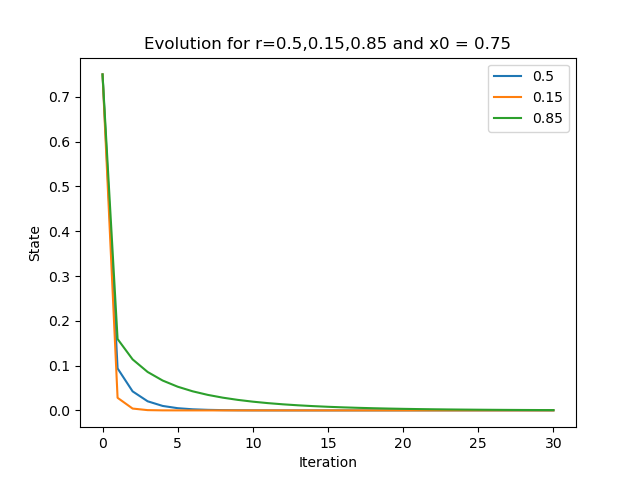
\includegraphics{Github_Repos/DataScience_for_Engineer_FA2023/Untitled Folder/figure2.png}

This is how the different graphs look at r=0.5,0.15, and 0.85 at x=0.75.
All these graphs do converge at zero at some point, but when r=0.15, it
converges the fastest.

\hypertarget{section-2}{%
\section{3.}\label{section-2}}

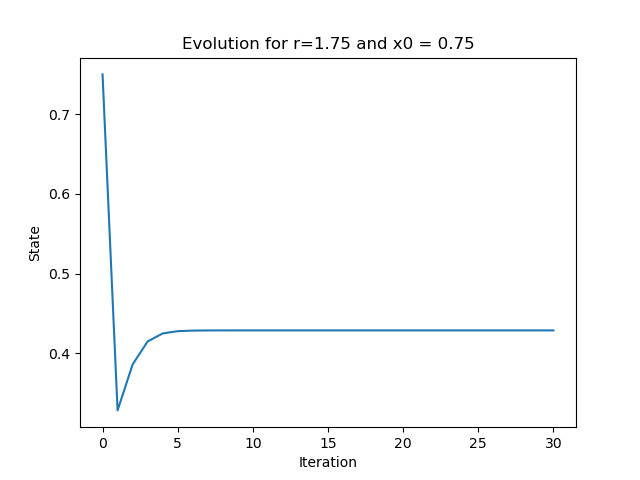
\includegraphics{Github_Repos/DataScience_for_Engineer_FA2023/Untitled Folder/figure3.png}

This graph shows the values of r=1.75 at x=0.75 over 31 iterations. with
this graph, we see that it immediately spikes down close to zero then
rises and converges around 0.4

\hypertarget{section-3}{%
\section{4.}\label{section-3}}

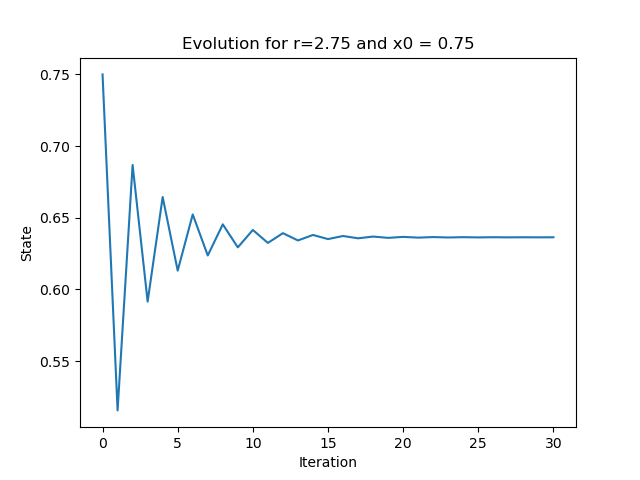
\includegraphics{Github_Repos/DataScience_for_Engineer_FA2023/Untitled Folder/figure4.png}

This graph shows the values of r=2.75 at x=0.75 over 31 iterations. With
this graph, we see that it fluctuates quite a bit until its 13
iteration, from there, it converges onto approximately 0.63

\hypertarget{section-4}{%
\section{5.}\label{section-4}}

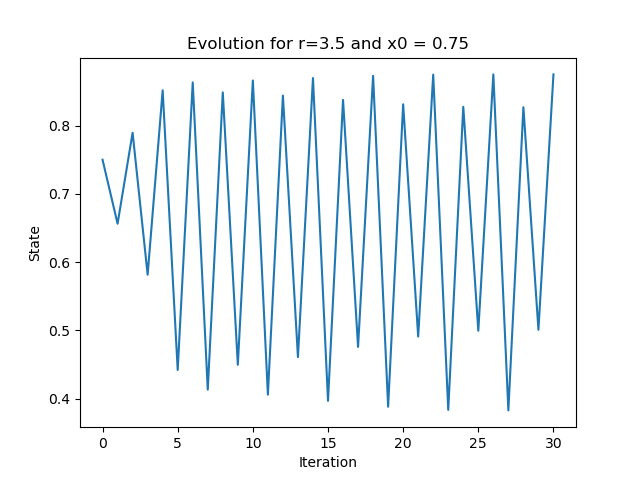
\includegraphics{Github_Repos/DataScience_for_Engineer_FA2023/Untitled Folder/figure5.png}

This graph shows the values of r=3.5 at x=0.75 over 31 iterations. With
this graph, we see that it fluctuates through all of its iterations,
reaching a maximum of 0.9 and a minimum of around 0.38 very
consistently. At this r value, it doesn't converge onto anything.

\hypertarget{section-5}{%
\section{6.}\label{section-5}}

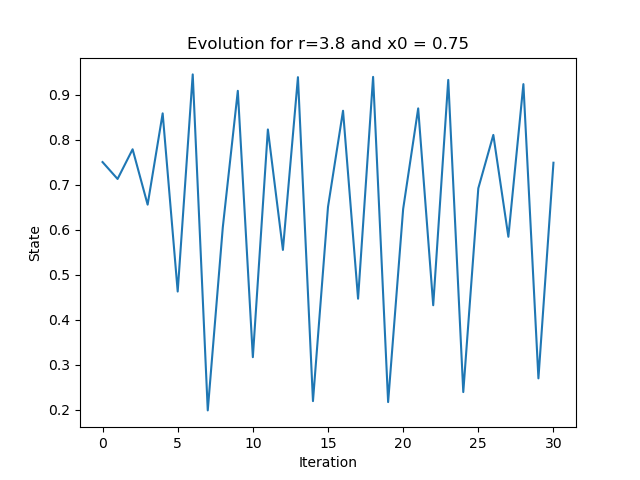
\includegraphics{Github_Repos/DataScience_for_Engineer_FA2023/Untitled Folder/figure6.png}

This graph shows the values of r=3.8 at x=0.75 over 31 iterations. With
this graph, we see that yet again it fluctuates very much, refusing to
converge onto a value

\hypertarget{section-6}{%
\section{7.}\label{section-6}}

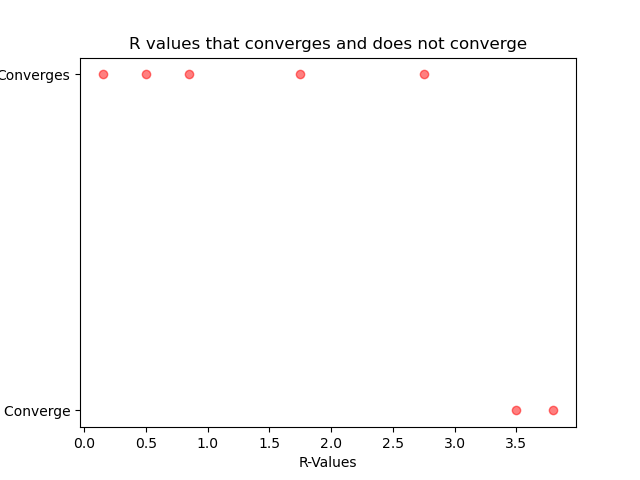
\includegraphics{Github_Repos/DataScience_for_Engineer_FA2023/Untitled Folder/figure7.png}

This graph shows what values of r converge and which ones don't
converge. We determine if a r value converges if x{[}1500{]} is less
than 10−7 in magnitude or if the absolute value of the difference of the
last two elements divided by the last element is less than 0.0001. From
the graph, I don't see any values that were previously stated not to
converge being marked converges or vice versa, which means that point
the previously plotted graphs and this graph are both reliable in
figuring it what values of r converge.

\hypertarget{section-7}{%
\section{8.}\label{section-7}}



\end{document}
